\documentclass[11pt]{article}

% ============================================================================
%  Life on air (P3), ISME Journal original article. Revised after review round 1 (12 October 2026).
%  Every number traces to lifeonair/results/ (README.md lists the producing script per folder);
%  corrected values are registered in notes/CORRECTIONS.md.
% ============================================================================

\usepackage[a4paper,margin=2.4cm]{geometry}
\usepackage[T1]{fontenc}
\usepackage{graphicx}
\usepackage{booktabs}
\usepackage{array}
\usepackage{authblk}
\renewcommand{\Authfont}{\normalsize}
\renewcommand{\Affilfont}{\small}
\usepackage{xcolor}
\usepackage{lineno}
\usepackage[numbers,sort&compress]{natbib}
\usepackage{hyperref}
\hypersetup{colorlinks=true,linkcolor=blue!50!black,citecolor=teal!60!black,urlcolor=blue!50!black}
\setlength{\emergencystretch}{2em}
\providecommand{\todo}[1]{\textcolor{red}{\textbf{[TODO: #1]}}}
\renewcommand{\thetable}{S\arabic{table}}

\title{\textbf{Group 1l hydrogen scavengers are relatively depleted beside plant roots across the
hyperarid Rub' al-Khali}}
% Author list and affiliations from ../empty-quarter-amplicon/main.tex.
% Alejandra first, Rund second, shared first authorship, per Robert, 13 October 2026.
\author[1]{Alejandra Lopez Velazquez\thanks{Alejandra Lopez Velazquez and Rund Tawfiq
  contributed equally and share first authorship.}}
\author[1]{Rund Tawfiq\textsuperscript{*}}
\author[1]{Marwa Abdelhakim}
\author[3]{Sulaiman M. Alajel}
\author[1]{Mohammed Alarawi}
\author[1]{Hind Aldakhil}
\author[1]{Abderahmane Derouiche}
\author[5]{Daniela I. Drautz-Moses}
\author[4]{Michel Dumontier}
\author[7]{Raik Grünberg}
\author[1]{Maxat Kulmanov}
\author[2]{Susana Martinez Arbas}
\author[1]{Kexin Niu}
\author[1]{Krishnakumar Sivakumar}
\author[6]{Tiannyu Wang}
\author[5]{Xiang Zhao}
\author[1]{Jood Kamal Zubair}
\author[6]{Magnus Rueping}
\author[1]{Robert Hoehndorf\thanks{Correspondence:
  robert.hoehndorf@kaust.edu.sa}}

\affil[1]{Bio-Ontology Research Group (BORG), Computer, Electrical and
  Mathematical Sciences and Engineering (CEMSE) Division, King Abdullah
  University of Science and Technology (KAUST), Thuwal, Saudi Arabia}
\affil[2]{Luxembourg Centre for Systems Biomedicine (LCSB), University of
  Luxembourg, Esch-sur-Alzette, Luxembourg}
\affil[3]{Ministry of Environment, Water and Agriculture, Saudi Arabia}
\affil[4]{Institute of Data Science, Department of Advanced Computing
  Sciences, Faculty of Science and Engineering, Maastricht University,
  Maastricht, The Netherlands}
\affil[5]{Bioscience Core Lab, King Abdullah University of Science and
  Technology, Thuwal, Saudi Arabia}
\affil[6]{Physical Science and Engineering (PSE) Division, King Abdullah
  University of Science and Technology (KAUST), Thuwal, Saudi Arabia}
\affil[7]{Biological and Environmental Science and Engineering (BESE)
  Division, King Abdullah University of Science and Technology (KAUST),
  Thuwal, Saudi Arabia}

\date{}

\begin{document}
\maketitle
\linenumbers

\section*{Abstract}
Desert soil bacteria can persist on atmospheric hydrogen and carbon monoxide, which they oxidise with
high-affinity enzymes. How the genes for these enzymes are distributed within and between desert
soils is known mainly from single-time transects and from studies that treat hydrogen oxidation as one
function. We typed the [NiFe]-hydrogenase and carbon monoxide dehydrogenase large subunits of 5{,}438
species-level genomes from the hyperarid Rub' al-Khali and quantified each group relative to single-copy
ribosomal genes in 546 shotgun metagenomes from 59 transect sites, sampled on up to five expeditions between
2023 and 2025 at the surface, in bulk soil at 5--10~cm and beside plant roots at the same depth.
Relative to bulk soil, root-adjacent soil had 4.8-fold lower relative group 1l hydrogenase representation
(106 paired site visits at 47 sites; lower in 89\%), 1.8 log$_2$ units more than the change in control
hydrogenases and carbon monoxide dehydrogenases; for groups 1h and 2a and form-I carbon monoxide
dehydrogenase, no change beyond the controls was detected. The relative depletion of group 1l was
larger in samples with higher extract DNA yield and arose almost entirely from turnover of genera, and
genera carrying group 1l were depleted beside roots beyond what their predicted growth potential and
phylogeny explained. Surface soil, in contrast, carried less of all four high-affinity groups than bulk
soil. Across sites, group 1l in bulk soil and all four groups at the surface were negatively associated
with long-term precipitation, but neither association was robust to both the choice of precipitation
product and spatial blocking. These patterns identify plant-associated relative exclusion of one
hydrogen-scavenging guild as a replicated feature of hyperarid soil, which measurements of biomass,
carbon and gas uptake can now test.

% ============================================================================
\section*{Introduction}
Soil bacteria oxidise hydrogen and carbon monoxide at their trace atmospheric concentrations, and
soil uptake is the largest sink of tropospheric hydrogen \citep{ehhalt2009h2cycle}. Hydrogen is
oxidised at atmospheric concentrations by group 1h and 1l [NiFe]-hydrogenases
\citep{greening2016genomic,ortiz2021antarctic} and also by some group 2a enzymes
\citep{islam2020group2a,grinter2023structural}; carbon monoxide is oxidised by the form-I carbon
monoxide dehydrogenase \citep{king2007coox,cordero2019atmospheric}. Genomes encoding these enzymes are
widespread in soil \citep{bay2021trace}, the energy they yield sustains dormant cells
\citep{greening2015persistence,cordero2019atmospheric}, and in deserts atmospheric oxidation can
contribute to primary production \citep{ji2017atmospheric,ray2022atmospheric}. Arid regions weigh
heavily in estimates of the soil hydrogen sink \citep{reji2025h2sink}, yet how the capacity for
trace-gas oxidation is distributed within a desert remains poorly resolved.

Three factors have been examined, each with a different design. Along aridity gradients sampled once,
the abundance of high-affinity hydrogenases and cell-specific hydrogen oxidation increased towards the
dry end in the Negev \citep{bay2021aridity}, and hydrogen oxidation per 16S rRNA gene copy was highest in
the most arid zone of the Namib \citep{tribbia2026namib}. Hydration experiments follow a single soil:
wetting desert soil decreased the relative abundance and expression of group 1l genes while stimulating
hydrogen uptake \citep{jordaan2020gobi}, and in another desert soil group 1l transcription increased
during hydration \citep{imminger2024resuscitation}. Plants, finally, concentrate organic carbon. In the
Mu Us Desert, genes for hydrogen and carbon monoxide oxidation were less abundant under shrubs than in
open soil, decreased with organic carbon and behaved as traits of oligotrophs whose uptake was suppressed
by added carbon \citep{li2023fertile}; most hydrogenases typed in that study belonged to groups 1d and
2a. Across many plant species, predicted maximal growth rate is a leading predictor of which bacteria
are enriched in the rhizosphere \citep{lopez2023rhizosphere}. Two questions remain open in hot sand
deserts, which are under-represented among genome-resolved surveys
\citep{ortiz2021antarctic,ray2022atmospheric,ray2023mmbr,hutchinson2025antarctic}: whether plants act on
all high-affinity groups or on particular ones, and whether such a pattern reflects the growth strategy
of the carriers, their phylogeny or the enzyme they carry.

We addressed these questions in the Rub' al-Khali, a hyperarid sand desert, using shotgun metagenomes
from 59 sites along a 1{,}043-km transect, sampled on up to five expeditions at three positions: the
surface, bulk soil at 5--10~cm and root-adjacent soil at the same depth. The depth-matched contrast
removes depth as a difference between root-adjacent and bulk soil, and repeated visits allow spatial
and within-site associations with precipitation to be estimated separately. We typed every hydrogenase
and carbon monoxide dehydrogenase large subunit in a catalogue of 5{,}438 species representatives and
quantified each group in reads, using non-high-affinity hydrogenases and carbon monoxide dehydrogenases
as controls that share the same normaliser. The analysis was exploratory. Our initial expectations, that
plants would enrich hydrogen scavengers and that wetter years would reduce them, were not supported, and
the questions below were formulated after inspecting the same data: whether the depletion of
hydrogen-scavenging capacity beside roots is specific to one enzyme group; whether it reflects biomass
scaling, lineage turnover or the growth strategy of the carriers; how the surface differs from bulk
soil; and how robust the association with long-term aridity is across sites and over time. We report
effect sizes with site-level uncertainty and control the false discovery rate within declared families
of tests.

% ============================================================================
\section*{Materials and methods}

\subsection*{Sampling, sequencing and genome catalogue}
Sampling, DNA extraction, sequencing and the genome catalogue are shared with companion papers on the
same transect\todo{cite the data descriptor and the MAG catalogue paper}. Sixty sites along a 1{,}043~km
west to east transect through the Saudi Rub' al-Khali were sampled on five expeditions (17--20 March
2023, 14 July 2023, 17--21 February 2024, 19--21 August 2024 and 12--15 October 2025). At each site and
visit, three co-located replicates were taken at three positions: surface soil (0~cm), bulk subsurface
soil (5--10~cm) and soil from the root zone of the nearest plant at 5--10~cm, which we call
root-adjacent because soil was not consistently attached to roots. Soil was frozen at $-20^\circ$C in the
field and stored at $-80^\circ$C. DNA was extracted from 0.9--1.2~g of soil with the QIAGEN PowerLyzer
PowerSoil or DNeasy PowerSoil Pro kit and sequenced on an Illumina NovaSeq 6000 (150-nt paired reads;
101-nt reads for the fourth expedition). Reads were quality-filtered with fastp v1.0.1
\citep{chen2018fastp}. Samples from two special-interest locations outside the repeated transect (sites
62 and 64) and samples without site metadata were excluded, so the analysis covers sites 1--60.

Each sample was assembled with MEGAHIT v1.2.9 \citep{li2015megahit} and binned with SemiBin2 v2.2.1
\citep{pan2023semibin2}; bins were refined with DAS\_Tool v1.1.7 \citep{sieber2018dastool}, assessed with
CheckM2 v1.1.0 \citep{chklovski2023checkm2}, and the 12{,}434 bins of at least medium quality
(completeness $\geq 50\%$, contamination $\leq 10\%$) were dereplicated with dRep v3.6.2
\citep{olm2017drep} at 95\% average nucleotide identity into 5{,}438 species representatives.
Representatives were classified with GTDB-Tk v2.7.2 \citep{chaumeil2022gtdbtk} against GTDB release 232
\citep{parks2022gtdb} and annotated with Bakta v1.12.0 \citep{schwengers2021bakta} and eggNOG-mapper
v2.1.13 \citep{cantalapiedra2021eggnog}. Relative abundance of each representative per sample was
computed with CoverM v0.7.0 \citep{aroney2025coverm} in genome mode. For 1{,}010 representatives that
refinement emitted as contig subsets of a parent bin, annotations were taken from the parent bin and
restricted to genes on contigs retained in the representative, matched by sequence; genes on removed
contigs were not counted towards carriage or traits.

\subsection*{Typing of hydrogenase and carbon monoxide dehydrogenase large subunits}
Proteins annotated with the [NiFe]-hydrogenase large subunit orthologue (KEGG K06281) and the carbon
monoxide dehydrogenase large subunit orthologue (K03520) were extracted from the representatives. Each
hydrogenase was assigned the class of its best DIAMOND blastp hit (\texttt{--ultra-sensitive}) in HydDB
\citep{sondergaard2016hyddb,greening2016genomic}. We analyse groups 1h, 1l and 2a separately, because all
three include enzymes that oxidise atmospheric hydrogen \citep{greening2016genomic,islam2020group2a}. Each
CoxL protein was called form I when it carried the form-I active-site motif AYXCSFR, including the
variants with S in the first or L in the sixth position reported among form-I references
\citep{imaura2026coxl}, and form II when it carried AYRGAGR
\citep{king2007coox,martincuadrado2009coxl,cunliffe2011roseobacter}; proteins without either motif were
called form I at more than 55\% identity and at least 90\% query coverage to the three form-I references of
\citet{cordero2019atmospheric} and were otherwise unresolved. All 59 form-I calls made without the motif were
fragments in which the alignment did not span the motif region. A representative carries a group when it
encodes at least one retained protein of that group.

To check the genomic context of typed genes, we took the ten genes on each side of every typed large
subunit on the same contig from the Bakta annotation and scored the co-occurrence of the hydrogenase
small subunit (K06282, K05927, K00437), hydrogenase maturation genes (K04651--K04656, K03605, K03192, or
Bakta product names) and, for CoxL, the medium and small subunits (K03519, K03518) and the accessory genes
\textit{coxDEFG}. Proportions are reported for loci with at least five genes on both sides; they describe
neighbourhood co-occurrence within the stated window.

For display, hydrogenase large subunits of at least 400 residues were clustered at 70\% identity with
MMseqs2 v18.8cc5c \citep{steinegger2017mmseqs2}, combined with all HydDB group 1 and group 2 references,
aligned with MAFFT v7.526 \citep{katoh2013mafft} (\texttt{--auto}), stripped of columns with more than 50\%
gaps and used to build a tree with FastTree v2.2.0 \citep{price2010fasttree} (\texttt{-lg -gamma}), rooted
on the clade that best separates the group 2 references. CoxL proteins of at least 600 residues were
treated in the same way with the form-I references.

\subsection*{Read-based quantification}
Groups were quantified in reads so that sequences outside the genome catalogue contribute. A competitive
protein database contained every typed hydrogenase large subunit of the representatives labelled with its
HydDB class, all HydDB reference hydrogenases, every CoxL protein of the representatives labelled form I,
form II or unresolved, the three form-I CoxL references, and 14 universal single-copy ribosomal proteins of
the representatives (KEGG K02886, K02906, K02926, K02931, K02933, K02867, K02874, K02878, K02982, K02988,
K02994, K02946, K02948 and K02965) clustered at 90\% identity. Every read is assigned to its single best
hit, so related enzymes of other classes compete for each read. From each sample, 10 million forward reads
were drawn with seqtk v1.5 \citep{li2023seqtk} (seed 11) and truncated to 100~nt so that the 101-nt and
150-nt libraries were screened identically; reads shorter than 75~nt were discarded. Reads were searched
with DIAMOND v2.0.15 \citep{buchfink2021diamond} blastx (\texttt{--id 50 --evalue 1e-5 --max-target-seqs
1}), and each read's best hit with an alignment of at least 25 residues was counted at identity floors of
50, 60 and 70\%. For each sample and label, reads were divided by the length of the hit subject in
kilobases and summed, and each marker was divided by the median of the 14 ribosomal-protein values. The
result, genome equivalents (GE), is an estimated ratio of marker to single-copy-gene coverage, which
approximates marker copies per genome \citep{nayfach2015microbecensus}; differences in read assignment
between markers and the ribosomal proteins offset it from true copies per genome (see the mock communities
below). GE describe relative gene representation among the genomes present. The primary
measure used the 60\% identity floor and samples in which at least 10 of the 14 ribosomal proteins were
detected.

We report six markers: group 1l, 1h and 2a hydrogenases, form-I CoxL, all other [NiFe]-hydrogenases and
all other CoxL (form II and unresolved). The last two serve as controls. Of the 573 sequenced samples
screened, 546 from sites 1--60 had complete metadata and passed the ribosomal-protein filter (116
surface, 164 bulk and 266 root-adjacent samples; median 9.77 million reads screened).

To estimate how well reads are assigned when their source is absent from the database, we tiled 100-nt
fragments every 30~nt over each typed gene and held out, in five folds each, (i) all marker proteins of
20\% of the representatives, (ii) 20\% of the clusters of catalogue marker proteins at 50\% identity, with
the HydDB and CoxL references retained, and (iii) 20\% of graph components, obtained by
single-linkage grouping of all marker proteins of the database, catalogue and references alike, at 70\%
identity over at least half of the shorter protein in a DIAMOND search ($E\leq10^{-5}$), with every member of a held-out component removed.
Fixed identity thresholds can assign reads of one enzyme class to a homologue \citep{orellana2017rocker},
and scheme (iii) tests removal of connected reference groups. A more permissive verification search
($E\leq10$) still found 34 of 6,478 held-out proteins with matches above 70\% identity at half-length
coverage (maximum 83.3\%); this benchmark therefore does not guarantee identity-disjoint references.
At a 50\% linkage
threshold, groups 1l and 1h formed a single component, and holding out that component reduced recall to near zero. Fragments
of 50 random non-marker genes per held-out genome were added as negatives, and fragments were classified
exactly as the reads. To calibrate GE, we simulated 20 communities from the CoverM profiles of bulk and
root-adjacent samples of ten site visits, drawing 4 million 150-nt reads with 0.5\% substitutions from the
representative genomes in proportion to their abundance and truncating them to 100~nt; true copies per
genome were the cell-weighted mean number of typed markers. The reads were screened against the full
database and against a database from which every marker and ribosomal protein of the community's own
genomes had been removed. The form-I CoxL misassignment rates of scheme (ii) were used to correct form-I
and other CoxL GE by inverting the $2\times2$ assignment matrix, as a sensitivity analysis.

\subsection*{Contamination screen}
Representatives whose GTDB genus matched a 16S rRNA amplicon variant flagged in 17
extraction blanks of the fifth expedition or six of the fourth expedition were flagged, and a re-implementation of the frequency method of
decontam \citep{davis2018decontam} compared abundance models independent of and inversely proportional to
extracted DNA concentration, both over all samples with a single recorded concentration and after centring
within each combination of expedition and extraction kit. Reads whose best hit belonged to a
representative flagged by either method were removed in a sensitivity analysis. The shotgun no-template
control of the fourth expedition contained no reads assigned to groups 1l, 1h or 2a or to form-I CoxL; its
only marker reads came from an \textit{Escherichia} genome carrying group 1c and 1d hydrogenases.
The fourth-expedition screen compared six blanks with 95 biological profiles and yielded seven candidate
variants (one-sided Fisher $p<0.1$, detection in at least two blanks and higher prevalence in blanks).
The three named genera, \textit{Alcaligenes}, \textit{Brevibacterium} and \textit{Nesterenkonia}, matched
14 representatives, four additional to the previous exclusion set; four variants lacked a named genus.
Candidate sequences and calls are retained with the analysis. The combined exclusion set contained 387
representatives, including two catalogue orphans already removed from the primary analysis.
These cross-assay genus matches define a conservative sensitivity screen and do not establish contamination
of individual MAGs. Genus, genome-trait and candidate carbon-fixation models were refitted after these
exclusions; their sensitivity estimates use model standard errors without repeating the site bootstrap.

\subsection*{Environmental covariates}
Daily precipitation for 1995--2025 was obtained from the ERA5 reanalysis \citep{hersbach2020era5} at
0.25$^\circ$ resolution through the Open-Meteo archive (\texttt{models=era5}). Long-term mean annual
precipitation was computed for 1995--2024 and, as sensitivity, from the NASA POWER 2001--2020 climatology
based on MERRA-2 \citep{gelaro2017merra2} and from Open-Meteo's default blend of ERA5 with the ECMWF
operational model. Mean annual precipitation from ERA5 ranged from 13 to 19~mm across sites; because
reanalysis precipitation in Saudi Arabia agrees only moderately with gauges \citep{wang2025sara}, we
treat it as a ranking of sites rather than an absolute water balance. The 60 sites fall into 41 ERA5 grid
cells. Antecedent precipitation was the sum over the 90 and 365 days before each site visit from ERA5 and,
as sensitivity, from NASA POWER daily data (MERRA-2 based) and the blended product (365 days, first four
expeditions). Surface skin temperature was the NASA POWER daily mean (TS) over the 30 days before the
centre date of each expedition, and soil moisture the SMAP surface value over the preceding 30 days. Vegetation greenness was the median MODIS normalised
difference vegetation index (NDVI; MOD13Q1 and MYD13Q1 v061, 250~m \citep{didan2021mod13q1}) over the 60
days before sampling. Extract DNA concentration was taken from the sample ledger for samples with a single
positive recorded value (267 of 546 samples). Soil geochemistry was summarised from X-ray fluorescence
measurements of the same sites by centred log-ratio principal components and by Ca, Cl and S. Soil organic
carbon and water content were not measured on these samples.

\subsection*{Statistical analysis}
Analyses were run in R v4.4.3 with lme4 v2.0.6 \citep{bates2015lme4}, vegan v2.7.5
\citep{oksanen2025vegan} and ape v5.8.1 \citep{paradis2019ape}. A site visit is one site sampled on one
expedition. For paired contrasts between positions, each marker was summarised as the median over
replicates within a site visit and the log$_2$ ratio of the medians computed for each visit with both
positions, with a pseudocount of 0.01~GE (results without a pseudocount and with 0.001 and 0.1 are
reported). Confidence intervals were obtained by resampling sites with replacement (2{,}000 resamples), and
tests are Wilcoxon signed-rank tests on site means of the visit values, so that the site is the
independent unit. The excess change of a high-affinity marker is its log$_2$ ratio minus the mean of the
two control log$_2$ ratios. A shared change in the ribosomal-protein denominator would shift all markers
equally, and the excess removes it up to the effects of the pseudocount and of taking replicate medians
separately for each marker. Mixed models of log$_2$ GE with marker, position, their interaction and
expedition as fixed effects and site, site visit and sample as random intercepts tested the interaction
by likelihood ratio. The contribution of position to each marker was summarised as the gain in marginal
$R^2$ when position is added to a model with expedition.

To relate group 1l to biomass, log$_2$ GE was regressed on log$_2$ extract DNA concentration with position,
expedition and extraction kit as fixed effects and site and site visit as random intercepts; the DNA term
was split into within-visit and between-visit components, the model was repeated within visits that used a
single kit and within bulk soil, each with extraction kit as a fixed effect and site and site visit as
random intercepts. If DNA concentration measured biomass with classical error of reliability 0.8 or 0.6,
the slope would be attenuated by that factor, and we report the correspondingly rescaled slopes as a
conditional sensitivity. Under a model in which group 1l copies per gram scale with biomass with exponent
$\alpha$, GE scale with exponent $\alpha-1$. The root effect on group 1l was estimated with and without the
DNA term in the same samples.

The change in the share of the mapped community held by group 1l carriers between root-adjacent and bulk
soil was decomposed into a genus-turnover term (change in genus abundance at the mean carrier fraction of
each genus) and a within-genus term (change in the carrier fraction of each genus at its mean abundance).
Genera absent from one position contributed zero abundance there, and the carrier fraction of a genus
present in only one position was taken from that position; the turnover share was bootstrapped over sites.
The same decomposition was applied across bulk-soil sites against mean annual precipitation, with genus
shares averaged over all visits to a site and absent genera counted as zero. Within the 81 genera that
contain both carriers and non-carriers, the logit of the carrier share of each genus at each site, clipped
to 0.005--0.995, was modelled on standardised log precipitation in a Gaussian mixed model weighted by the
square root of the genus share, with genus and site as random intercepts; clipping at 0.001 and 0.02 is
reported. To separate the number of carriers from the number of copies per
carrier, the root contrast was computed for the abundance share of carriers ($F$), their copy-weighted share
($M$) and copies per carrier ($C$).

For growth strategy, the minimum doubling time of each representative was predicted from codon usage bias
with gRodon2 v2.7.3 \citep{weissman2021grodon} in partial mode from coding sequences of at least 240~nt
with ribosomal-protein genes as the highly expressed set; these are predictions of maximal growth
potential under the codon-usage model. Doubling time, completeness-adjusted genome size and GC content were
compared between carriers and non-carriers in mixed models with order as a random intercept. The
community-weighted mean log doubling time of a sample was the CoverM-weighted mean over representatives
with an estimate, and its shift between root-adjacent and bulk soil was computed per site visit. The
mapped abundance with a doubling-time estimate was a median of 97--99\% per position (lowest 1.5\%), and the
analysis was repeated in samples with at least 80\% and 90\% coverage and with unestimated representatives
set to the fastest or the slowest observed doubling time. The
excess change of group 1l was regressed on this shift with site and expedition as random intercepts, and
the intercept, which estimates the excess at zero shift, was bootstrapped over sites. Across genera with a
mean bulk-soil share of at least 0.05\% of the mapped community, the median visit-level log$_2$ ratio
between root-adjacent and bulk soil was regressed on median log doubling time and the fractions of
representatives carrying groups 1l, 1h and 2a and form-I CoxL, with phylum as a fixed effect and weights
equal to the square root of the bulk-soil share; the model was repeated for genera with a nonzero ratio,
for genera with at least two representatives, for genera present in at least 25\% or 50\% of paired visits,
with carriage computed among representatives at least 90\% complete, and with order instead of phylum as a
fixed effect, and the group 1l coefficient was bootstrapped over sites by recomputing the genus ratios from
resampled visits. As a candidate screen for co-carriage of carbon fixation, genomes encoding all three
Calvin--Benson--Bassham marker orthologues (RuBisCO large and small subunits, K01601 and K01602, and
phosphoribulokinase, K00855) were compared between group 1l and 1h carriers in a binomial mixed model with
order as a random intercept, with and without genome completeness and among genomes at least 90\% complete.

Spatial associations were Spearman correlations of site medians with mean annual precipitation for each
position, marker and precipitation product, with each site entered once and confidence intervals from a bootstrap over $k$-means spatial blocks of the site
coordinates ($k = 4, 6, 8, 10$), Moran's $I$ of the residuals with inverse-distance weights, and partial
correlations controlling for latitude, longitude and elevation, for the first two geochemical principal
components, for Ca, Cl and S, and for the first principal coordinate of community composition. A mixed
model over all samples regressed log$_2$ GE on standardised log precipitation with position and expedition
as fixed effects and site and site visit as random intercepts. For change over time, log antecedent
precipitation was split into a within-site component and a site mean, and log$_2$ visit medians were
modelled on both with expedition as a fixed effect and site as a random intercept; the within-site slope
was bootstrapped over sites and scaled to the within-site interquartile range of precipitation, and an
interval was compared with an exploratory bound of $\pm 0.5$ log$_2$(GE+0.01) units.
This bound corresponds to a factor of $\sqrt{2}$ on the pseudocount-shifted GE scale; its ecological
interpretation is weakest for sparse markers. The exposure scale is the pooled interquartile range
of within-site deviations of log(1+precipitation). The within-site estimates were repeated with ERA5 and NASA POWER exposures, with a
bootstrap over ERA5 grid cells instead of sites, leaving out each expedition in turn and with pseudocounts
of 0.001 and 0.1. These intervals are conditional on the available climate grids and do not propagate
local rainfall measurement error; bootstrap fits with finite estimates were retained without a full
convergence audit. Because the surface exposure models rest on 68 visits in which temperature was largely
determined by expedition, they were repeated leaving out each expedition. Turnover of composition was
partitioned by PERMANOVA \citep{anderson2001permanova} on Bray--Curtis dissimilarities between visit-level
profiles (mean relative abundance over the replicates of a site, expedition and position) at sites visited
at least twice, with whole visit profiles permuted among expeditions within each site and position; the
dispersion test used the same permutation design. The Benjamini--Hochberg procedure
\citep{benjamini1995fdr} was applied within each declared family: the ten quantities (six markers and four
excess changes) of each position contrast; the twelve spatial correlations (three positions by four groups)
for each precipitation product; the twelve within-site slopes for each antecedent-precipitation exposure;
and the twelve surface exposure models (four groups by three exposures). Genus, DNA, NDVI,
genome-trait and carbon-fixation co-occurrence models are exploratory; their reported $p$ values are
unadjusted. Sensitivity variants assess dependence on analysis choices within these same data.

Sensitivity variants recomputed the position contrasts and spatial correlations at identity floors of 50
and 70\%, without reads to contamination-flagged representatives, without reads to the 122 group 1l
proteins typed below 50\% identity or 80\% coverage to their HydDB hit, with motif-less form-I CoxL calls
treated as unresolved, with CoxL GE corrected for misassignment, without the fifth and without the fourth
expedition. The excess of group 1l was also computed against each control separately.

% ============================================================================
\section*{Results}

\subsection*{Group 1l is the most abundant high-affinity hydrogenase in Rub' al-Khali soil}
Of the 5{,}438 species representatives, 597 encode a group 1l, 410 a group 1h and
134 a group 2a hydrogenase, and 245 a form-I CoxL (Fig.~\ref{fig:guilds}a,
Fig.~\ref{fig:coxl}). In loci with at least five genes on each side (445 group 1l, 224 group 1h, 53 group 2a
and 125 form-I CoxL loci), a small-subunit gene co-occurred with 73\% of group 1l, 84\% of group 1h and all
group 2a large subunits, and maturation genes with 87\%, 96\% and 100\%; the medium and small CoxL subunits
co-occurred with 96\% of form-I CoxL. In bulk soil, the median sample carried 1.08 group 1l copies per genome
equivalent, 0.14 group 1h, 0.03 group 2a and 0.11 form-I CoxL.

Read-assignment performance depended on the relatives retained in the database (Table~\ref{tab:benchmark}). With clusters of catalogue proteins defined at 50\% identity held out and external references retained, 89\% of group 1l fragments were assigned to group 1l, 99\% of group
1h, 94\% of group 2a and 82\% of form-I CoxL fragments to their own group, although only 77\% of fragments
called form I came from form-I genes. When every database protein linked to the source at 70\% identity was
removed, recall fell to 66\% for group 1l, 44\% for form-I CoxL and 23\% for group 2a, but fragments called
group 1l still came from group 1l in 92\% of cases; group 1h recall was near zero because its references were held out together with group 1l, and 14\% of its fragments were called group 1l. Recall of
group 1l was similar across the twelve orders tested (55--73\%). Of fragments from non-marker genes, 2 of 1.5
million (cluster scheme) and 16 of 1.3 million (component scheme) were assigned to group 1l. In 20 simulated communities built from the abundance profiles
of bulk and root-adjacent samples, GE exceeded true copies per genome by a median of 0.67 log$_2$ units for
group 1l, 0.80 for group 1h, 0.60 for group 2a, 0.84 for form-I CoxL and 1.11 for other CoxL, but tracked
them closely (Pearson $r$ on the log scale 0.93--1.00; Table~\ref{tab:mock}). Because the offset was
similar in both positions, the root-to-bulk ratio of group 1l was recovered with a mean error of $-0.11$
log$_2$ units (largest 0.41; $-0.05$ and 0.48 when the community's own genomes were removed from the
database), against an observed ratio of $-2.27$. The other-[NiFe] control, in contrast, was nearly absent
from the simulated genomes but estimated at 0.02--0.13 GE from off-target assignment, so we also report
the excess of group 1l against other CoxL alone.

\subsection*{Root-adjacent soil carries less group 1l relative to other genes}
We compared root-adjacent and bulk soil in the 106 site visits at 47 sites where both were sampled at
5--10~cm. Group 1l GE were lower beside roots by a median of 2.27 log$_2$ units, a 4.8-fold difference (95\%
CI $-2.90$ to $-1.59$; lower in 89\% of visits; $p=3\times10^{-7}$; Fig.~\ref{fig:guilds}b). The control
hydrogenases and CoxL were lower by 0.40 and 0.28 units, and the excess change of group 1l beyond the
controls was $-1.83$ ($-2.62$ to $-1.00$; $q=2\times10^{-6}$); against other CoxL alone it was $-1.81$ and
against other [NiFe]-hydrogenases alone $-1.98$. For groups 1h ($-0.01$; 95\% CI $-0.22$ to $0.14$), 2a
($-0.02$; $-0.20$ to $0.25$) and form-I CoxL ($-0.05$; $-0.19$ to $0.14$), no change beyond the controls was
detected (all $q>0.8$; Fig.~\ref{fig:guilds}d); these intervals exclude a group 1l-sized excess but not
smaller changes. In the mixed model,
marker and position interacted ($\chi^2=324$, 5 df), and only the group 1l interaction departed from the
reference ($-1.75$, SE 0.12; other high-affinity groups between $-0.08$ and $+0.07$). Position accounted for
a gain in marginal $R^2$ of 0.22 for group 1l and 0.02--0.10 for the other markers.

The difference was consistent across expeditions, analysis choices and lineages. The excess change of group
1l was negative in each expedition ($-0.99$ to $-2.63$), between $-1.54$ and $-1.85$ in every sensitivity
variant and between $-1.60$ and $-1.83$ against other CoxL alone (Table~\ref{tab:sensitivity}), and $-1.82$ without a pseudocount and $-1.32$ with a pseudocount of
0.1. All ten orders of group 1l carriers with the highest share of bulk soil had a lower share beside roots
(Table~\ref{tab:lineages}).

\subsection*{The depletion of group 1l scales with DNA yield and with genus turnover}
Copies per genome equivalent fall either when carriers decline or when other organisms increase. Extract
DNA concentration, a proxy that combines microbial biomass with extraction efficiency and plant DNA, was a
median 10-fold higher in root-adjacent than in bulk soil (log$_2$ ratio 3.37, 47 visits). Across 267
samples, group 1l GE fell by 0.32 log$_2$ units (SE 0.03) per doubling of DNA concentration, within visits
($-0.30$) as well as between them ($-0.35$), within visits extracted with a single kit ($-0.34$) and within
bulk soil alone ($-0.20$, SE 0.05). Groups 1h and 2a ($-0.02$ and $-0.03$, SE 0.02) did not detectably scale
with DNA, and the controls scaled only weakly (other [NiFe] $-0.034$, SE 0.009; other CoxL $-0.032$, SE 0.012;
Fig.~\ref{fig:scaling}a). Under the scaling model the group 1l slope corresponds to an exponent of about
0.7: if DNA concentration tracked biomass, group 1l copies per gram would increase less than proportionally
with biomass. In the same 214 root-adjacent and bulk samples, adding DNA concentration to the model reduced
the root effect on group 1l from $-2.12$ (SE 0.23) to $-1.36$ (SE 0.20; Fig.~\ref{fig:scaling}c), a
conditional attenuation of 36\%. The DNA-adjusted coefficient describes the position contrast
at a given extract concentration. Its biological interpretation depends on the contributions of
microbial biomass, plant DNA and extraction efficiency to that concentration.

The change was carried by lineage composition. The share of the mapped community held by group 1l
carriers fell from a median of 0.31 in bulk soil to 0.06 beside roots, and genus turnover accounted for
97\% of this change (site bootstrap 96.7--98.3\%); the within-genus term was small ($-0.005$ per visit)
although consistently negative ($p<0.001$). The share of carriers fell by 2.17 log$_2$ units, their copy-weighted share by 2.30 and
the number of copies per carrier by only 0.19 (105 visits), so the depletion reflects fewer carrier genomes rather than
fewer copies in each.

\subsection*{Genera carrying group 1l are depleted beyond their predicted growth potential}
Root-adjacent communities had shorter predicted doubling times than bulk soil in 79\% of 106 visits
(community-weighted log doubling time $-0.26$; $p=1.4\times10^{-5}$), consistent with the enrichment of
taxa with high predicted growth rates in rhizospheres \citep{lopez2023rhizosphere}. Within orders, carriers of
group 1l ($+0.12$, SE 0.03), group 1h ($+0.12$) and group 2a ($+0.20$) had longer predicted doubling times
than non-carriers, so a shift towards organisms with shorter predicted doubling times would be expected to
deplete all three groups. Only group 1l, however, was depleted beyond the controls. The excess change of
group 1l was larger where the community shifted more ($\rho=$0.26; slope 1.73, SE 0.61), and at zero shift
the model still predicted an excess of $-1.57$ (site bootstrap $-2.22$ to $-0.93$; Fig.~\ref{fig:scaling}c).
The intercept was stable when samples with less than 80\% or 90\% of mapped abundance covered by
doubling-time estimates were removed ($-1.56$, $-1.48$) and when unestimated representatives were assigned
the slowest ($-1.54$) or the fastest observed doubling time ($-1.97$), but the slope was not: with the
fastest assignment it fell to 0.23 (SE 0.45), so the association between the growth shift and the excess
depends on how unestimated genomes are treated.

Across 289 genera, the fraction of a genus carrying group 1l predicted its depletion beside roots ($-0.81$
log$_2$ units, SE 0.18; site bootstrap $-1.12$ to $-0.52$) with predicted doubling time, carriage of the
other groups and phylum in the model, whereas carriage of group 1h and form-I CoxL did not
(Fig.~\ref{fig:scaling}b). The association held among genera with a nonzero ratio ($-0.92$), with at least
two representatives ($-1.08$), present in at least 25\% or 50\% of paired visits ($-1.12$, $-1.18$), with
carriage counted among genomes at least 90\% complete ($-0.98$) and with order instead of phylum as a fixed
effect ($-1.03$, SE 0.22). With order in the model, predicted doubling time no longer predicted genus
depletion ($-0.05$, SE 0.15), and carriage of group 2a also did ($-1.68$, SE 0.67; 134 carriers), although
group 2a showed no excess depletion at the community level. Finer phylogenetic control therefore shifts
weight from predicted growth potential to lineage. Vegetation greenness was negatively associated
with group 1l in bulk soil ($-0.80$ log$_2$ units per standard deviation of NDVI, SE 0.19) and at the surface
($-1.17$, SE 0.16) with mean annual precipitation in the model, and the excess change beside roots was
smaller at greener sites (site medians, $\rho=0.37$, 47 sites).

Group 1l carriers also differed in genome traits. Within orders, they had higher GC content than
non-carriers (+0.7 percentage points) and genomes of similar size ($-1.9\%$, $p=0.08$), whereas group 1h,
group 2a and form-I CoxL carriers had larger genomes (+7\%, +11\% and +17\%). Across all genomes, carriers
of group 1l only had a smaller median estimated genome size than genomes without high-affinity groups
(3.78 against 3.97~Mb), consistent with the across-lineage comparison of trace-gas oxidisers along a
northern-China aridity gradient \citep{wang2025genomesize}; that study used broader functional groups
and a different growth-prediction method. Our genome-size difference did not persist within orders. In a candidate screen for
carbon fixation, all three Calvin--Benson--Bassham marker genes were encoded by 18\% of group 1l-only and
8\% of group 1h-only carriers; the difference was not significant within orders (log-odds 0.73, SE 0.39,
$p=0.06$) but was after adjustment for genome completeness (0.96, $p=0.02$) and among genomes at least 90\%
complete (28\% against 9\%; 1.29, SE 0.54, $p=0.02$). RuBisCO co-occurs with high-affinity hydrogenases in
desert genomes worldwide \citep{leung2025aridity}. These comparisons describe candidate gene co-occurrence;
sequence-form and pathway validation would refine their functional interpretation. Excluding contamination-flagged
representatives retained the negative genus association for group 1l (281 genera; phylum-adjusted coefficient
$-0.77$, SE 0.18; order-adjusted $-0.96$, SE 0.21). The completeness-adjusted carbon-fixation association
also remained positive (log-odds 1.04, SE 0.43). With the expanded exclusion set, the median
root-to-bulk group-1l contrast was $-2.29$ log$_2$ units and its excess was $-1.76$ (106 visits at 47 sites).

\subsection*{The surface carries less of all high-affinity groups than bulk soil}
The surface contrast differed in kind from the root contrast. In 68 visits at 36 sites, all four
high-affinity groups were lower at the surface than in bulk soil beyond the controls: group 1l by 0.83
log$_2$ units, group 1h by 0.42, group 2a by 0.22 and form-I CoxL by 0.24 (all $q<0.02$;
Fig.~\ref{fig:guilds}c,d). Root-adjacent soil therefore differed from the surface by a lower excess of group
1l ($-0.85$) and a higher excess of group 1h ($+0.41$; 84 visits). At the surface, the excess change of
group 1h was less negative after warmer 30-day periods (1.76 log$_2$ units per standard deviation of skin
temperature, $q=0.001$), that is, the surface depletion of group 1h was weaker in warm seasons, while
associations with soil moisture and antecedent precipitation were not significant after correction.
Expedition explained 96\% of the variation in temperature among these 68 visits (residual standard deviation
1.3 against 6.3$^\circ$C), so this association mainly contrasts expeditions; it remained positive when each
expedition was left out in turn (1.08 to 2.56).

\subsection*{Spatial associations with aridity depend on the precipitation product}
Across 51 sites, group 1l GE in bulk soil were negatively associated with mean annual precipitation from
ERA5 ($\rho=-0.40$, $q=0.007$), NASA POWER ($-0.43$) and the blended product ($-0.51$).
The ERA5 association persisted after adjustment for geography ($-0.36$) and geochemistry ($-0.30$),
but its spatial block bootstrap intervals included zero at every block count (six blocks: $-0.64$ to
$0.07$; Fig.~\ref{fig:scaling}d). With POWER the intervals included zero at eight and ten blocks;
with the blended product they excluded zero at all four block counts. Adjustment for community composition
reduced the ERA5 correlation to $-0.02$.

At the surface, all four groups were negatively associated with ERA5 precipitation ($\rho=-0.46$ to
$-0.53$, 45 sites), with spatial block intervals below zero. For group 1l, however, the correlation
was weaker with POWER ($-0.29$, $q=0.078$) and the blended product ($-0.25$, $q=0.14$), whose block
intervals included zero. Residual spatial autocorrelation remained in the ERA5 models for group 1l
(Moran's $I=0.16$, $p<0.001$) and form-I CoxL ($p=0.046$). These associations therefore depend on
both the precipitation product and spatial structure.

The bulk-soil association also tracked lineage composition. Holding the carrier fraction of each genus
at its mean reproduced the correlation of the carrier share with precipitation ($-0.43$ for both the
observed and turnover-only shares). Within the 81 genera containing carriers and non-carriers, the
Gaussian model of clipped logits gave a negative carrier-share slope ($-0.29$ per standard deviation of
log precipitation, SE 0.12); changing the clipping threshold gave slopes of $-0.38$ and $-0.21$.

\subsection*{Within-site change between expeditions}
The five expeditions span 31 months. In bulk soil, the within-site association of group 1l with
precipitation over the preceding year was imprecise (103 visits at 35 sites; ERA5 $q=0.34$).
Resampling ERA5 grid cells gave an interval of $-0.03$ to $1.02$ log$_2$(GE+0.01) units across the
within-site interquartile range of log precipitation, and leaving out individual expeditions gave
estimates from $-0.32$ to $0.80$ (Fig.~\ref{fig:temporal}).

At the surface and beside roots, group 1l was lower after wetter 90-day periods according to ERA5
(changes of $-0.65$ and $-0.73$ log$_2$(GE+0.01) units; $q=0.013$ and $0.020$). These estimates
remained negative under grid-cell resampling, alternative pseudocounts and omission of each expedition.
With POWER exposures on the same visits, the estimates were $-0.12$ and $+0.33$, with intervals
spanning zero. Within-site 90-day precipitation anomalies agreed weakly between products
($\rho=0.19$ across 244 site visits), compared with $0.61$ for annual anomalies. The seasonal
association is therefore conditional on the precipitation product. Several other marker intervals
lay within the exploratory $\pm0.5$ bound on log$_2$(GE+0.01); their interpretation depends on the
pseudocount and exposure range.

In the visit-level community profiles, expedition accounted for 2.1\% of variation, site for 30.4\%
and position for 4.5\%. Permuting visits within site and position gave $p=0.001$ for expedition,
with dispersion also differing ($p=0.002$). Within bulk soil alone, expedition accounted for 3.7\%
($p=0.036$; dispersion $p=0.26$). The community profiles document temporal change, while inference
about rainfall responses is limited by the exposure products and the sparse repeated-site design.

% ============================================================================
\section*{Discussion}
Across 47 sites and five expeditions, root-adjacent soil carried a smaller relative representation of
group 1l hydrogenase genes than bulk soil at the same depth. This was the only high-affinity group with
a detectable excess depletion beyond the controls. The association persisted when other CoxL was used
as the sole control, when contamination-flagged references were excluded and across identity thresholds.
In the recovered catalogue, genus turnover accounted for most of the change, and genus carriage of
group 1l remained associated with depletion after adjustment for predicted growth potential and order.

The closest precedent is the depletion of trace-gas oxidation genes under shrubs in the Mu Us Desert
\citep{li2023fertile}. That study combined carbon measurements, amendments and gas uptake to link the
pattern to carbon availability. Our data add a replicated, group-resolved contrast in which the
additional depletion is concentrated in group 1l. Carbon responses differ between substrates and enzyme
groups: sucrose suppressed hydrogen uptake and group 1h gene copies in soil microcosms, whereas a low
cellulose dose stimulated uptake \citep{baril2023carbon}; in \textit{Mycobacterium smegmatis}, glycerol
repressed the group 2a hydrogenase Huc through GylR, while group 1h was outside that regulatory response
\citep{kropp2026glycerol}. Extending these comparisons to group 1l would test whether carbon regulation
contributes to its distinct distribution.

Predicted growth potential is a leading correlate of rhizosphere enrichment
\citep{lopez2023rhizosphere}. Root-adjacent communities in this study also had shorter predicted doubling
times, but the association between that shift and group 1l depletion depended on how genomes without
growth predictions were treated. The genus-level association with group 1l persisted under finer
phylogenetic control. Together with the turnover partition, this points to ecological differences
between lineages carrying group 1l. Hydrogenase genes can also move between lineages: frequent transfer
of groups 1l and 1h has been reported in Antarctic soil communities \citep{peng2026hgt}.
Hydration produced contrasting group 1l transcriptional responses in two desert soils
\citep{jordaan2020gobi,imminger2024resuscitation}. Moisture, oxygen and carbon availability therefore
remain candidate correlates of the root-associated pattern.

Extract DNA concentration supplies a further constraint on this interpretation. Group 1l representation
decreased as DNA concentration increased, and conditioning on DNA concentration attenuated the root
coefficient by 36\%. The result is compatible with group 1l carriers increasing less than proportionally
as other organisms increase beside roots. DNA concentration includes microbial and plant DNA and
extraction effects; calibrated gene copies or cells per gram would distinguish absolute changes from
changes in relative representation. Relative and quantitative rhizosphere profiles can differ in
direction \citep{azarbad2022relative}.

The surface had a broader depletion of high-affinity groups than root-adjacent soil. Its associations
with long-term and antecedent precipitation were strongest with ERA5 and weaker with POWER and the
blended product. The recent-temperature association chiefly compared expeditions and indicated weaker
group 1h depletion in warmer periods. In bulk soil, the precipitation gradient was also sensitive to
spatial blocking and community composition. ERA5 mean annual precipitation spans only 13--19~mm here,
and reanalysis rainfall in Saudi Arabia has substantial uncertainty \citep{wang2025sara}. These data
therefore resolve the depth-matched root contrast more consistently than they resolve precipitation
responses within this narrow hyperarid range.

The design measures relative gene representation in extracted DNA. Simulations of catalogue communities
recovered the group 1l root-to-bulk contrast with modest error despite biased absolute GE calibration;
communities containing more divergent genomes would provide a stronger test of generalisation.
The high GC content of group 1l carriers also makes library-dependent coverage bias relevant
\citep{browne2020gcbias}. Extracellular DNA can persist in dry soil
\citep{carini2016relicdna,lennon2018relicdna}; the available propidium-monoazide-treated amplicon pairs
cover two sites and only surface and root-adjacent soil. NDVI and predicted growth potential provide
indirect information about carbon supply at a root microsite. Direct carbon and water measurements,
calibrated biomass and gas-uptake measurements in paired root-adjacent and bulk soil would test the
proposed explanations independently. The hypotheses and secondary analyses in this study are
exploratory because they were formulated after inspection of these data.

% ============================================================================
\section*{Data and code availability}
The shotgun reads are deposited at the European Nucleotide Archive under study PRJEB125153 (public release
scheduled for 1 November 2026)\todo{confirm release date and sample accessions}. The species representatives
and their annotations are released with the companion catalogue paper. The analysis scripts, compact input
and output tables, figure code and an R environment specification are at
\url{https://github.com/bio-ontology-research-group/empty-quarter-lifeonair} in the folder \texttt{lifeonair/};
per-sample read counts are retrieved by the repository's large-file script, which checks them against a
checksum manifest. Bulk inputs remain on IBEX and require institutional access\todo{archival DOI before submission}.

\section*{Acknowledgements}
\todo{funding and acknowledgements}

\section*{Competing interests}
The authors declare no competing interests.

\bibliographystyle{unsrtnat}
\bibliography{references}

% ============================================================================
\clearpage
\begin{figure}[p]\centering
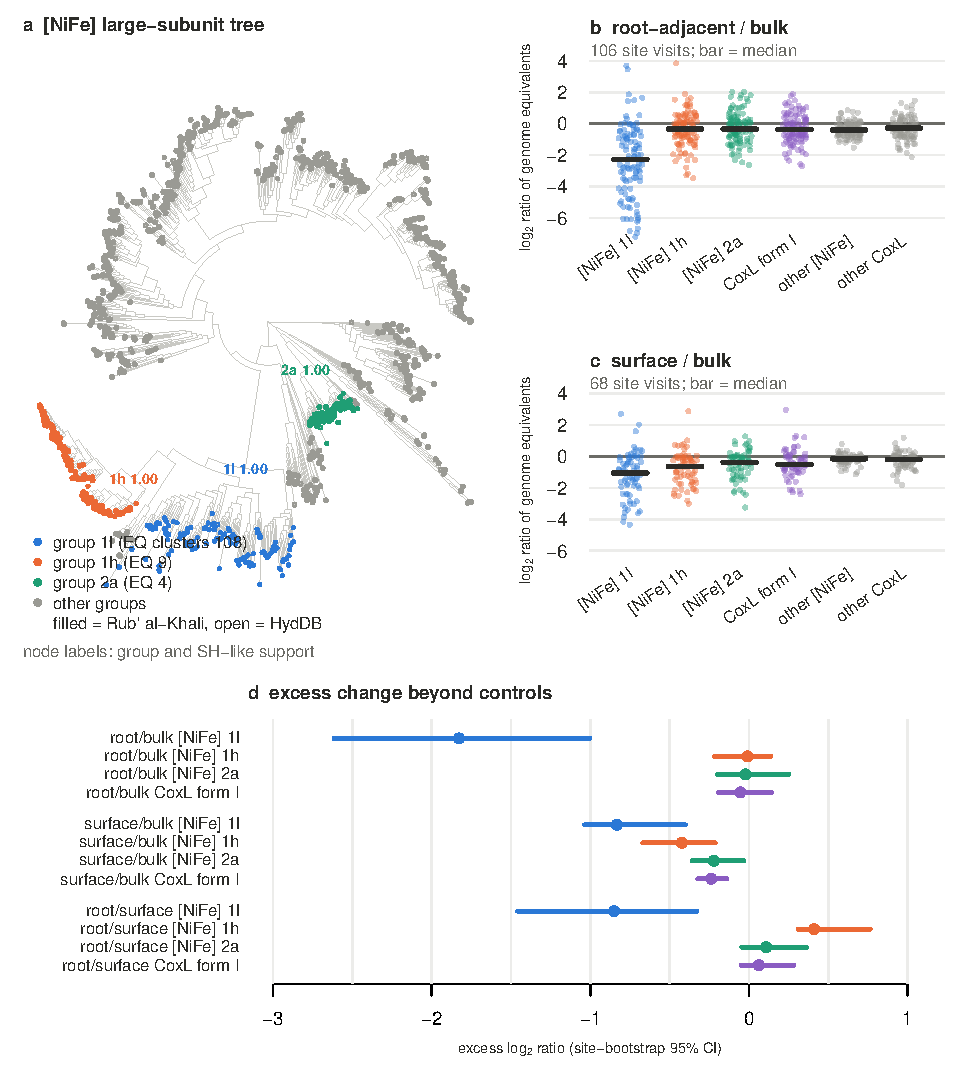
\includegraphics[width=\textwidth]{../figures/fig1_guilds.pdf}
\caption{\textbf{Root-adjacent soil carries less group 1l relative to other genes, and the surface carries
less of all high-affinity groups.} \textbf{a}, Tree of [NiFe]-hydrogenase large subunits from the Rub'
al-Khali catalogue (70\% identity cluster representatives, filled) and HydDB group 1 and 2 references
(open), rooted on group 2; group 1l blue, 1h orange, 2a green. \textbf{b}, Log$_2$ ratio of genome
equivalents in root-adjacent to bulk soil, both at 5--10~cm, per site visit (106 visits at 47 sites), for
the high-affinity groups and the two control marker sets; bars are medians. \textbf{c}, The same for surface
(0~cm) against bulk soil (68 visits at 36 sites). \textbf{d}, Excess log$_2$ ratio of each high-affinity
group beyond the mean of the two controls, median with 95\% confidence interval from resampling sites.}
\label{fig:guilds}
\end{figure}

\begin{figure}[p]\centering
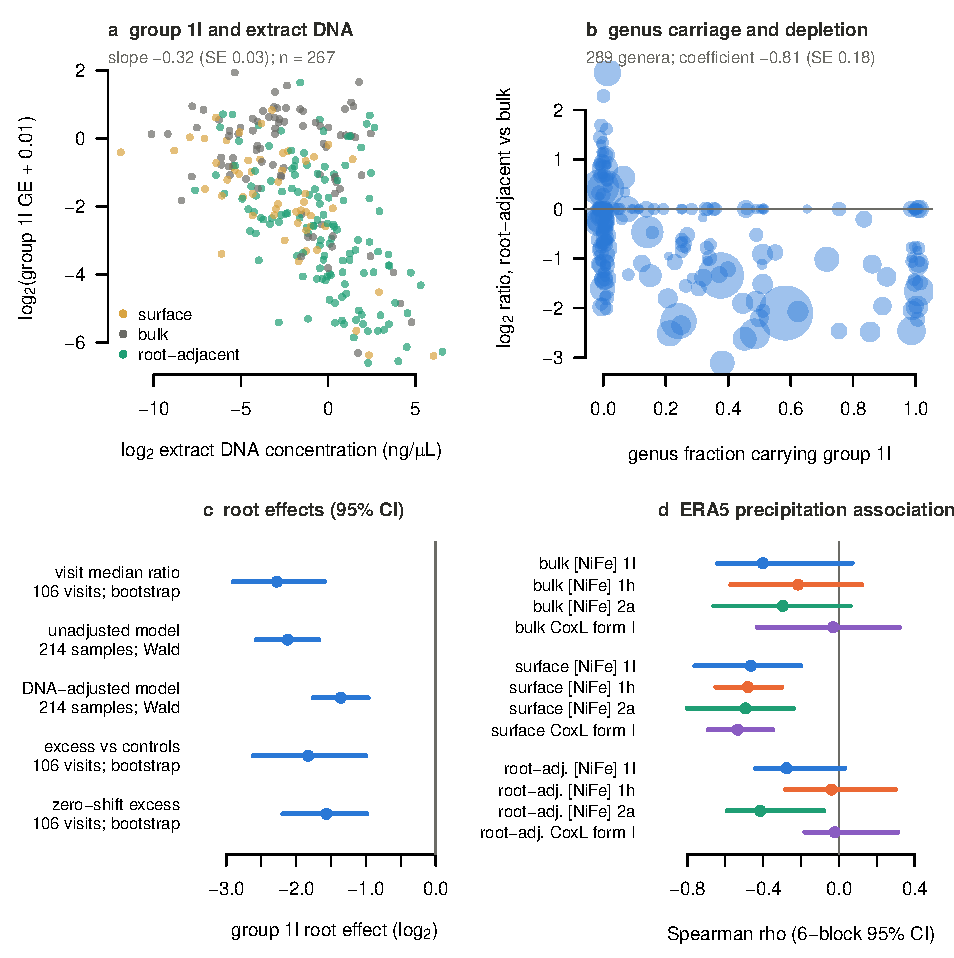
\includegraphics[width=\textwidth]{../figures/fig2_scaling.pdf}
\caption{\textbf{The relative depletion of group 1l scales with DNA yield and with genus carriage, and its
association with ERA5 precipitation varies by position.} \textbf{a}, Group 1l genome equivalents against
extract DNA concentration, per sample, coloured by position, with the mixed-model slope annotated. \textbf{b}, Median
log$_2$ ratio of genus abundance between root-adjacent and bulk soil against the fraction of the genus's
representatives carrying group 1l; symbol area scales with the genus's share of bulk soil; the coefficient
is from a weighted regression with predicted doubling time, carriage of the other groups and phylum.
\textbf{c}, Root effect on group 1l: the median visit log$_2$ ratio, the mixed-model estimate without and
with DNA concentration, the excess beyond the controls, and the excess predicted at zero shift in community
growth potential, with 95\% intervals. \textbf{d}, Spearman correlation of site medians with ERA5 mean
annual precipitation per position and group, with intervals from a bootstrap over six spatial blocks.}
\label{fig:scaling}
\end{figure}

% ============================================================================
\clearpage
\section*{Supplementary material}

\begin{table}[h]\centering\small
\caption{\textbf{Held-out benchmark of read assignment.} Fraction of 100-nt fragments from held-out genes
assigned to their own group (recall) and fraction of fragments assigned to a group that came from it
(precision), at the 60\% identity floor, when all marker proteins of 20\% of the representatives (genome)
or 20\% of catalogue 50\%-identity clusters were removed with external references retained, or
20\% of all-reference 70\%-identity components were removed, over five folds. Component linkage
required at least half-length coverage. A more permissive verification search found 34 held-out proteins
with matches above 70\% identity at this coverage, reaching 83.3\%; the holdout is not strictly identity-disjoint.}
\label{tab:benchmark}
\footnotesize
\begin{tabular}{lrrrrrr}
\toprule
Group & Recall & Precision & Recall & Precision & Recall & Precision\\
 & \multicolumn{2}{c}{Genome holdout} & \multicolumn{2}{c}{Catalogue cluster} & \multicolumn{2}{c}{All-reference component}\\
\midrule
\csname @@input\endcsname tab_benchmark.tex
\bottomrule
\end{tabular}
\end{table}

\begin{table}[h]\centering\small
\caption{\textbf{Calibration in 20 simulated catalogue communities.} True median marker copies per genome,
median log$_2$ GE bias, Pearson correlation on the log scale, and mean root-to-bulk log$_2$ ratio error
(number of evaluable pairs). Full: complete reference database. Removed: community genomes' marker and
ribosomal proteins removed. Simulation assumes uniform coverage and catalogue-only genomes.}
\label{tab:mock}
\footnotesize
\begin{tabular}{lrrrrrrr}
\toprule
 & True & \multicolumn{3}{c}{Full} & \multicolumn{3}{c}{Removed}\\
Group & copies & Bias & $r$ & Ratio error ($n$) & Bias & $r$ & Ratio error ($n$)\\
\midrule
\csname @@input\endcsname tab_mock.tex
\bottomrule
\end{tabular}
\end{table}

\begin{table}[h]\centering\small
\caption{\textbf{Sensitivity of the position contrasts and the spatial association.} Median log$_2$ ratio of
group 1l genome equivalents between root-adjacent and bulk soil, the excess beyond the controls with its
site-level Wilcoxon $p$, the excess for group 1h and form-I CoxL, group 1l excess against other CoxL alone, the surface excess of group 1l, and the
Spearman correlation of bulk-soil site medians of group 1l with ERA5 and NASA POWER mean annual
precipitation.}
\label{tab:sensitivity}
\footnotesize\setlength{\tabcolsep}{4pt}
\begin{tabular}{lrrrrr}
\toprule
Variant & Samples & 1l ratio & 1l excess & $p$ & 1l vs CoxL\\
\midrule
\csname @@input\endcsname tab_sensitivity.tex
\bottomrule
\end{tabular}

\medskip
\begin{tabular}{lrrrrr}
\toprule
Variant & 1h excess & Form-I excess & Surface 1l & $\rho$ ERA5 & $\rho$ POWER\\
\midrule
\csname @@input\endcsname tab_sensitivity_secondary.tex
\bottomrule
\end{tabular}
\end{table}

\begin{table}[h]\centering\small
\caption{\textbf{Orders of group 1l carriers beside roots.} The ten orders of group 1l carriers with the
highest mean share of the mapped community in bulk soil, with the median log$_2$ ratio of their share
between root-adjacent and bulk soil over 106 site visits and the fraction of visits with a lower share
beside roots.}
\label{tab:lineages}
\begin{tabular}{llrrr}
\toprule
Phylum & Order & Bulk share (\%) & Log$_2$ ratio & Visits lower\\
\midrule
\csname @@input\endcsname tab_lineages.tex
\bottomrule
\end{tabular}
\end{table}

\begin{figure}[h]\centering
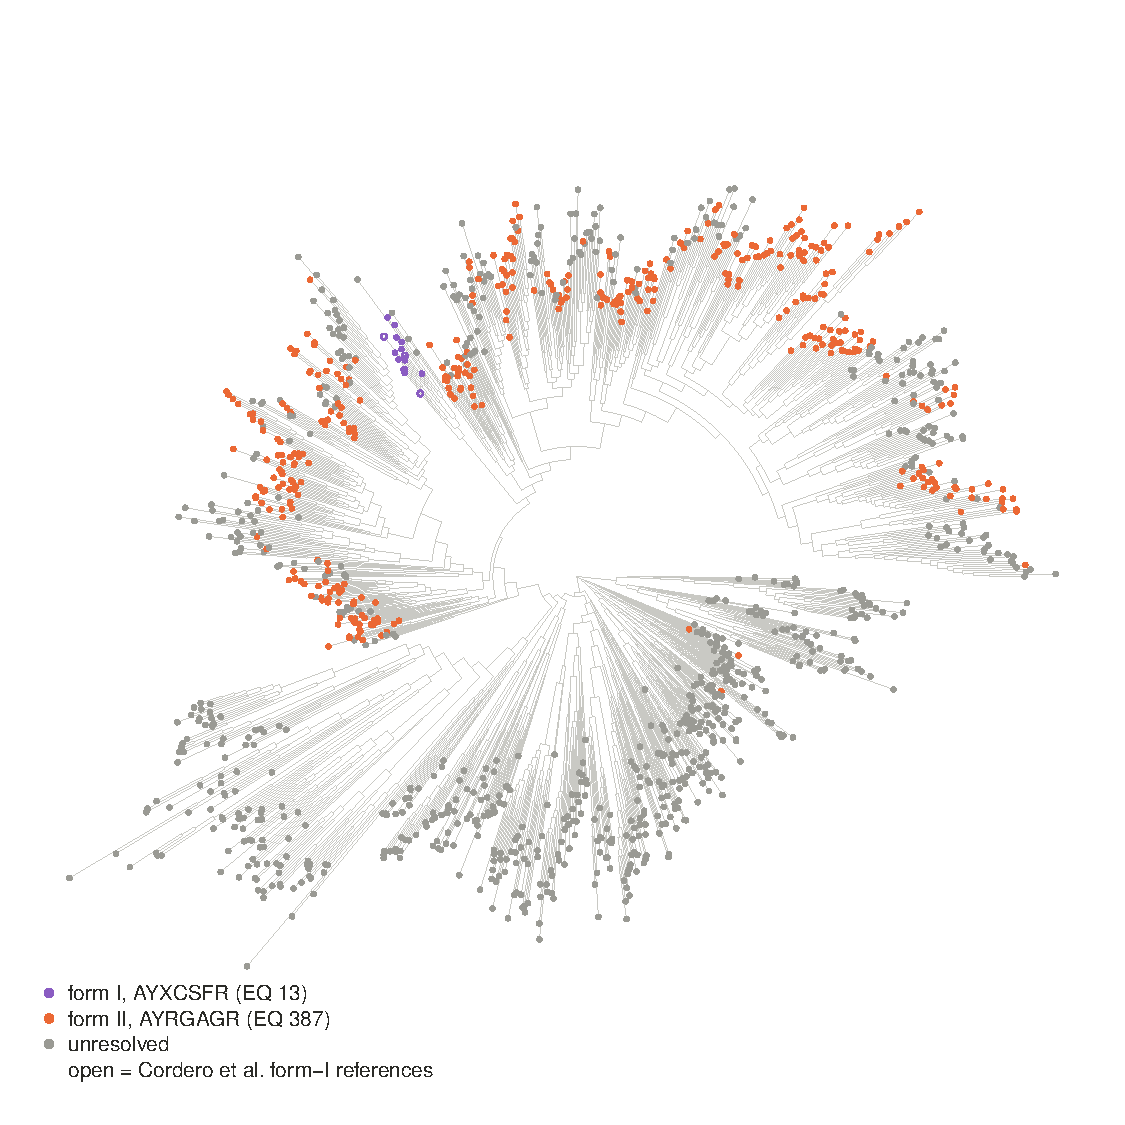
\includegraphics[width=\textwidth]{../figures/figS1_coxL_tree.pdf}
\renewcommand{\figurename}{Supplementary Figure}
\renewcommand{\thefigure}{S1}
\caption{\textbf{CoxL large subunits.} Tree of Rub' al-Khali CoxL proteins of at least 600 residues (70\%
identity cluster representatives, filled) with the three form-I references of \citet{cordero2019atmospheric}
(open). Form I (AYXCSFR and specified variants) purple, form II (AYRGAGR) orange, unresolved grey.}
\label{fig:coxl}
\end{figure}

\begin{figure}[h]\centering
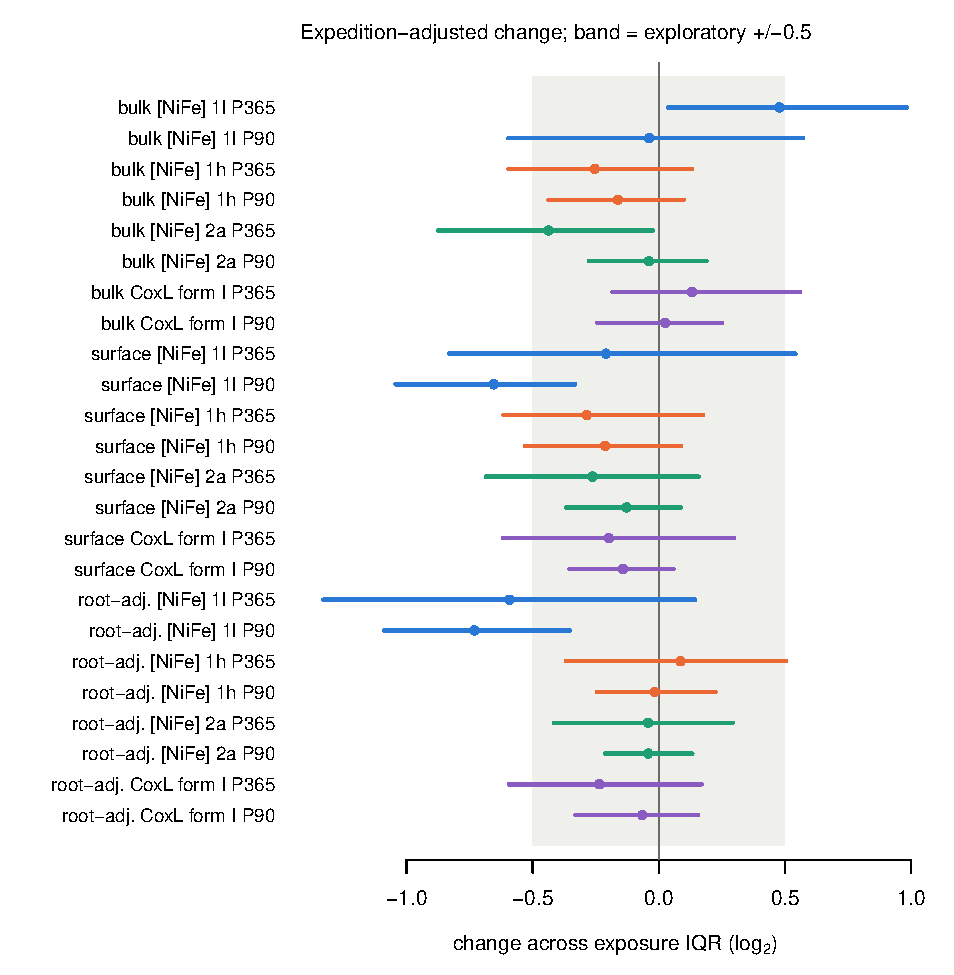
\includegraphics[width=\textwidth]{../figures/figS2_temporal.pdf}
\renewcommand{\figurename}{Supplementary Figure}
\renewcommand{\thefigure}{S2}
\caption{\textbf{Within-site change between expeditions.} Change in log$_2$(GE+0.01) across the
within-site interquartile range of log(1+antecedent ERA5 precipitation) over 90 and 365 days, from mixed models
with expedition as a fixed effect and site as a random intercept, with 95\% intervals from resampling
sites. The shaded band marks the exploratory $\pm 0.5$ bound on the transformed scale.}
\label{fig:temporal}
\end{figure}

\end{document}
